\myChapter{Proposition d'un langage permettant d'exprimer les politiques d'accès basé sur la hiérarchie organisationnelle et les attributs}{}\label{chapLangage}

\myMiniToc{section}{Contenu} 

\mySection{Introduction}{}\label{sectionIntroduction}

Dans ce chapitre, il sera question pour nous de proposer une extension du langage XACML afin d'exprimer de façon fine granulaire des politiques de notre modèle. Notre chapitre est structuré comme suite: nous présenterons d'une part le langage XACML et ces concepts de base et d'autre part nous proposerons une extension de ce langage afin d'exprimer des règles d'accès basées non seulement sur des attributs mais aussi sur la hiérarchie organisationnelle d'une organisation.


\mySection{Langage de balisage extensible de contrôle d'accès}{}\label{sectionXACML}

\mySubSection{Présentation de XACML}{}\label{sectionpresentationXACML}

XACML (eXtensible Access Control Markup Language) est une spécification normalisée par l'OASIS \cite{standard13, anderson03, godik02}. Il s'agit d'un langage XML dédié au contrôle d'accès. Il inclut un langage protocolaire de type requêtes/réponses pour la prise de décision et un langage pour la définition de politiques de contrôle d'accès \cite{abakar12}. \\
%\hspace*{0.5cm} Le langage de balisage de contrôle d'accès extensible reste le seul moyen standardisé d'appliquer dynamiquement l'autorisation en externalisant les contrôles d'accès des applications et des bases de données et en utilisant des politiques commerciales - dans ce que l'on appelle également le contrôle d'accès basé sur les attributs (ABAC) pour déterminer qui peut accéder à quelles données sous conditions multiples et fines. À la base, il se compose d'un langage standard, d'un protocole de réponse/requête et d'une architecture de référence.\\
%\hspace*{0.5cm}Dans la norme XACML 3.0 Oasis \cite{standard13}, il est indiqué que ; « S'il est mis en œuvre dans toute une entreprise, un langage de politique commun permet à l'entreprise de gérer l'application de tous les éléments de sa politique de sécurité dans toutes les composantes de ses systèmes d'information. La gestion de la politique de sécurité peut inclure certaines ou toutes les étapes suivantes : rédiger, réviser, tester, approuver, publier, combiner, analyser, modifier, retirer, récupérer et appliquer la politique. »

\mySubSection{Architecture du langage XACML}{}\label{sectionArchitectureXACML}

L'architecture XACML est composée de cinq modules logiciels clés qui fonctionnent à l'unisson pour appliquer une autorisation d'exécution normalisée à chaque point de demande d'accès.

\mySubSubSection{Point d'administration des politiques (PAP)}{}\label{sectionArchitectureXACMLPAP}

Le point d'administration des politiques est le point de rédaction des politiques. Une fois qu'un utilisateur a écrit ou modifié/mis à jour une politique en langage clair, le PAP la convertit automatiquement en code XAML lisible par machine et basé sur des normes pour l'administration et l'application par le système.

\mySubSubSection{Point d'information politique (PIP)}{}\label{sectionArchitectureXACMLPIP}

Le point d'information de politique est un système puissant qui appelle les différents répertoires d'attributs et services tiers au moment de l'exécution afin que le point de décision de politique établisse si la demande répond aux spécifications d'une politique. Ces soi-disant valeurs d'attribut comprenant la ressource, la source, l'environnement, etc.

\mySubSubSection{Point de récupération des politiques (PRP)}{}\label{sectionArchitectureXACMLPRP}

Le point de récupération de politique est le point de stockage des politiques d'autorisation d'accès XACML. Il s'agit le plus souvent d'un système de fichiers ou d'une base de données.

\mySubSubSection{Point de décision politique (PDP)}{}\label{sectionArchitectureXACMLPDP}

Le point de décision de politique évalue la demande, en fonction de ce qui est écrit dans une politique, et prend une décision – généralement Autoriser ou Refuser l'accès. Le PDP XACML informe alors le PEP de la décision.

\mySubSubSection{Point d'application des politiques (PEP)}{}\label{sectionArchitectureXACMLPEP}

Le point d'application de la politique reçoit la demande d'accès et applique la décision d'autorisation ou de refus du PDP XACML au moment de l'exécution.

\mySubSection{Flux d'autorisation XACML}{}\label{sectionFluxXACML}

Les principaux acteurs du domaine XACML sont présentés dans le diagramme de flux de données de la figure \ref{figflux}. \\

\begin{figure}[h!]
    \centering
		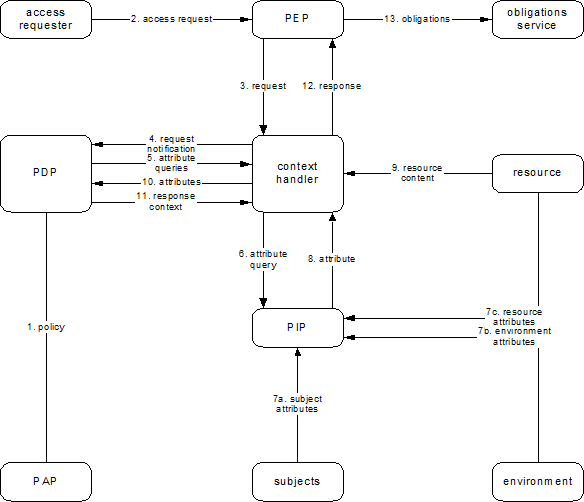
\includegraphics[scale=4.9]{chap4/images/fluxDonnee.png}
    \caption{Diagramme de flux de données \cite{standard13}}
	 \label{figflux}
\end{figure} 

\hspace*{0.5cm} Le modèle fonctionne selon les étapes suivantes \cite{standard13}.
\begin{enumerate}
\item Les PAP rédigent des politiques et des ensembles de politiques et les mettent à la disposition du PDP. Ces politiques ou ensembles de politiques représentent la politique complète pour une cible spécifiée;
\item Le demandeur d'accès envoie une demande d'accès au PEP;
\item Le PEP envoie la demande d'accès au gestionnaire de contexte « context handler » dans son format de demande natif, incluant éventuellement les attributs des sujets, ressource, action, environnement et d'autres catégories;
\item Le gestionnaire de contexte construit un contexte de demande XACML, ajoute éventuellement des attributs et l'envoie au PDP;
\item Le PDP demande tous les attributs sujet, ressource, action, environnement et autres catégories (non représentés) supplémentaires au gestionnaire de contexte;
\item Le gestionnaire de contexte demande les attributs d'un PIP;
\item Le PIP obtient les attributs demandés;
\item Le PIP renvoie les attributs demandés au gestionnaire de contexte;
\item Facultativement, le gestionnaire de contexte inclut la ressource dans le contexte;
\item Le gestionnaire de contexte envoie les attributs demandés et (éventuellement) la ressource au PDP. Le PDP évalue la politique;
\item Le PDP renvoie le contexte de réponse (y compris la décision d'autorisation ) au gestionnaire de contexte;
\item Le gestionnaire de contexte traduit le contexte de réponse au format de réponse natif du PEP. Le gestionnaire de contexte renvoie la réponse au PEP;
\item Le PEP remplit les obligations;
\item (Non représenté) Si l'accès est autorisé, alors le PEP autorise l'accès à la ressource; sinon, il refuse l'accès.

\end{enumerate}

\mySubSection{Structure et syntaxe du langage XACML }{}\label{sectionStructureXACML}

Le langage de politique XACML est composé d'un certain nombre d'éléments clés qui permettent d'implémenter une autorisation précise sur différents modèles de déploiement, c'est-à-dire des environnements Cloud, sur site et hébergés.

\mySubSubSection{Cible }{}\label{sectionCible}

XACML a introduit la notion cible « Target» afin d'identifier les règles et les politiques qui
concernent une requête. La cible est composée d'attributs qui décrivent le sujet, les
ressources, les actions et l' l'environnement:
\begin{itemize}
\item \textbf{Le sujet} décrit les attributs de l'utilisateur qui a fait une demande d'accès;
\item \textbf{La ressource} décrit les attributs de l'objet auquel l'accès est demandé;
\item \textbf{L'action} représente les attributs qui décrivent les mesures que le sujet veut
prendre sur la ressource demandée;
\item \textbf{L'environnement} concerne les attributs détenant des informations sur le
contexte.
\end{itemize}

\hspace*{0.5cm} Chacun de ces composants est déterminé par des propriétés. Un sujet peut être défini
par un identificateur, un groupe auquel il appartient, un rôle etc. Une ressource peut être caractérisée par un identificateur, des propriétés et un type. La même chose pour l'action qui peut être définie par un identificateur, le nom d'action à effectuer. Par exemple, nous considérons la requête suivante: \\
\hspace*{0.5cm} Un étudiant identifie par « user-id» qui appartient au groupe « A» veut accéder à un document public en mode écriture. Pour cette requête nous pouvons distinguer:

\begin{itemize}
\item Le sujet: user-id ;
\item La ressource: document public;
\item L'action: écriture.
\end{itemize}

\hspace*{0.5cm} Les propriétés des sujets, ressources et actions sont appelées attributs. Chaque attribut
possède une valeur. Une cible permet au PDP XACML de vérifier quelle stratégie ou quelles règles s'appliquent à une certaine demande. Les instructions de cible agissent comme des définisseurs pour les attributs pertinents de la règle, de la stratégie ou de l'ensemble de stratégies.

\mySubSubSection{Règle}{}\label{sectionRègle}

Une règle de contrôle d'accès est définie avec le langage XACML comme étant un ensemble de prédicats qui répondent aux questions suivantes \cite{errachid11}:
\begin{itemize}
  \item Quels sont les sujets concernés?
  \item Quelles sont les ressources demandées?
  \item Quelles sont les actions demandées?
  \item Quelle est la décision à renvoyer?
  \end{itemize}
  
 \hspace*{0.5cm} Une règle XACML est composée d'un effet, d'une cible et d'une condition:
 \begin{itemize}
 \item effet: détermine la décision de la règle. C'est soit « Permit» soit «Deny» ;
 \item cible: permet de déterminer si la règle correspond à la requête ou non;
 \item condition: décrite par un prédicat sur les attributs de la règle.
\end{itemize}  
 
%Une règle est un composant de base d'une stratégie. En tant que tel, il fournit l'effet souhaité de la politique - autoriser ou refuser. Une règle peut contenir une cible, une condition, un conseil ou un ensemble d'obligations.

\mySubSubSection{Politique }{}\label{sectionPolitique}

Une politique est exprimée par une cible, un ensemble de règles et un algorithme de
combinaison \cite{errachid11}. Pour identifier les politiques appropriées à l'évaluation de la requête, il faut d'abord comparer la cible de la règle avec la cible de la politique, et par la suite, vérifier les conditions des règles de la politique afin de déterminer la décision « permit» ou « deny ». Il est possible que les règles d'une politique retournent des décisions différentes par rapport à une requête donnée. L'algorithme de combinaison des règles permet de spécifier comment déterminer la décision de la politique.
Les décisions possibles sont \cite{standard13}:
\begin{itemize}
\item \textbf{Permit:} l'accès est autorisé;
\item \textbf{Deny:} l'accès à la ressource est refusé;
\item \textbf{lndeterminate:} il n'est pas possible d'appliquer la politique à la requête parce qu'un
élément (sujet, ressource, etc) est inconnu ou parce que la construction de la politique
ne permet pas d'aboutir à une décision (erreur) ;
\item \textbf{NotApplicable:} il n'est pas possible d'appliquer la politique à la requête car eUe ne
contient aucune règle qui s'applique à la requête.
\end{itemize}

\hspace*{0.5cm} \textbf{Un ensemble de Politiques} (Policyset) est une agrégation de plusieurs politiques ou des ensembles de politiques. Policyset contient aussi un algorithme de combinaison pour combiner la décision de politiques. 

%Une politique se compose d'une ou d'un ensemble de règles, d'un algorithme de confirmation de règle ainsi que d'obligations facultatives et d'un avis. La politique est la base à partir de laquelle le PDP XACML peut fonctionner.

\mySubSubSection{Algorithme de combinaison}{}\label{sectionAlgo}

Nous rappelons qu'un algorithme de combinaison permet de calculer la décision d'une politique et d'un ensemble de politiques à partir des décisions de leurs agrégats. XACML 2.0 offre quatre algorithmes de combinaison prédéfinis \cite{anderson03} :
\begin{itemize}
\item Permit-overrides: s'il y a une règle évaluée avec effet « Permit» alors la
décision de combinaison donne également un effet « permit» ;
\item Deny-overrides : s'il y a une règle évaluée avec effet « Deny» alors la
décision de combinaison donne un effet « Deny » ;
\item First-applicable : avec l'algorithme First-applicable, l'ordre d'évaluation des
règles est important. La politique prend l'effet de la première règle qui
s'applique (on ignore la règle non applicable);
\item Only-one-applicable : si plusieurs règles sont applicables, la décision
<<1ndeterminate» est retournée, sinon la décision de la politique est celle de la
règle applicable.
\end{itemize}

\hspace*{0.5cm} Une extension de ces algorithmes est ajoutée dans la version XACML 3.0, par exemple:

\begin{itemize}
\item Ordered-deny-overrides utilise le même principe que l'algorithme «Deny-override», sauf que l'ordre dans lequel les règles sont évaluées est le même que l'ordre dans lequel elles sont décrites dans la politique. La même chose pour l'algorithme « Ordered-permit-overrides »;
\item Deny-unless-permit est destiné pour les cas où une décision « Permit» doit avoir la priorité par rapport à la décision « Deny» et qu'aucune règle ne retourne la décision « lndeterminate ou NotApplicable ». Cet algorithme est particulièrement utile dans une structure politique et qu'un PDP retournera toujours une décision «permit ou deny » ;
\item est conçu pour les cas où une décision « Deny » devrait avoir priorité sur une décision « Permit ». 
\end{itemize}

\mySubSubSection{Ensemble de règles}{}\label{sectionEnsemble}

Un jeu de règles est un groupe de règles pouvant se trouver à divers emplacements. Les ensembles de politiques comprennent des politiques, un algorithme de combinaison de politiques, des obligations facultatives et un avis.

\mySubSubSection{Les conditions }{}\label{sectionCondition}

Les conditions font partie d'une règle et peuvent comparer les valeurs d'attributs, pour évaluer si un attribut est "vrai", "faux" ou "indéterminé". Dans l'exemple XACML ci-dessous, vous pouvez voir le rôle d'une condition lors de la vérification si le nom d'utilisateur d'un sujet est le même que l'attribut de propriétaire d'une ressource.

\begin{figure}[h!]
    \centering
		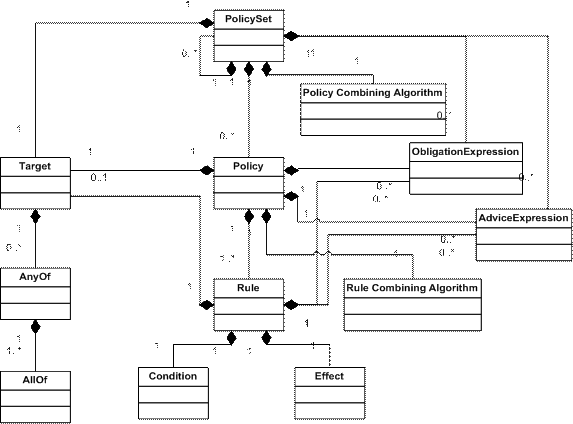
\includegraphics[scale=4.9]{chap4/images/model.png}
    \caption{Model du langage XACML \cite{standard13}}
	 \label{figflux}
\end{figure} 

\mySubSection{Avantages et inconvénient du langage XACML}{}\label{sectionAvantageXACML}

L'utilisation de XACML offre de nombreux avantages aux entreprises et aux grandes organisations qui ont besoin d'un moyen standardisé de partager des actifs en toute sécurité, tout en respectant et en prouvant la conformité.
\begin{itemize}

\item \textbf{Système géré de manière centralisée:} avec un référentiel central pour toutes les politiques XACML, XACML normalise l'autorisation pour fournir un contrôle inégalé des actifs dans l'entreprise à chaque point d'accès, que ce soit via une API, des micro-services, une application, un portail, un service Web ou une base de données;

\item \textbf{Éviter la dépendance vis-à-vis d'un fournisseur:} l'utilisation d'un langage basé sur des normes par opposition à un système propriétaire offre plus de flexibilité aux développeurs et évite la dépendance vis-à-vis des fournisseurs;

\item \textbf{Une sécurité à laquelle vous pouvez faire confiance:} la norme de politique XACML a été développée en collaboration et mise en œuvre par des experts en sécurité informatique de premier plan dans certaines des plus grandes entreprises mondiales. Il répond aux normes de sécurité les plus élevées;

\item \textbf{Création simplifiée de politiques:} pour simplifier l'écriture de stratégie dans XACML, des scripts JSON sont utilisés. Le format d'échange de données léger est facile à lire et à écrire pour les humains et facile à analyser et à générer pour les machines.
\end{itemize}

\mySection{Extension du langage XACML pour l'expression des politiques basé sur hiérarchie organisationnelle et les attributs}{}\label{sectionHXACL}

\mySubSection{Insertion du parapheur électronique dans l'architecture du langage XACML}{}\label{sectionParapheur}

\mySubSubSection{Le parapheur électronique }{}\label{sectionParapheurE}

%Ici il est question pour nous de présenter l'architecture de notre langage en intégrant dans l'architecture du langage XACML notre parapheur électronique
%Comme nous l'avoir vu dans le chapitre précédant, la parapheur électronique représente l'élément centrale de notre modèle car c'est celui-ci qui est chargé de l'interception des requêtes  des employés, puis les transmet au processus d'émission pour une évaluation 

Dans notre langage le parapheur électronique est composé des composants suivantes:
\begin{itemize}
\item \textbf{PEP:} Ce composant est charge de l'interception des requêtes des utilisateurs et de les envoyer au PDP pour une validation, puis il est chargé d'appliquer les décisions d'accès sur les ressources et d'envoyer;
\item \textbf{PDP:} Le point de décision de politique évalue la demande, en fonction de ce qui est écrit dans une politique, et prend une décision. Puis informe alors le PEP de la décision. 
\item \textbf{Le module de Traitement Hiérarchique (Treatment Hierarchical):} Il est chargé du contrôle hiérarchie de toutes les requêtes entrantes du système et ceci après validation de ces requêtes par le PDP
\end{itemize}

\mySubSubSection{Policy administration point }{}\label{sectionParapheurE} C'est le point de rédaction des politique de contrôle d'accès il peut être un éditeur de polices d'accès

\mySubSubSection{Policy information point }{}\label{sectionParapheurE} Il a  pour rôle d'extraire les informations supplémentaires qui ne sont pas présentes dans la demande d'accès. Le PIP peut lui-même chercher les informations dans des sources externes. Ces sources externes peuvent être une base de données.

\mySubSubSection{Polycy provider }{}\label{sectionParapheurE}
 Il est le point de stockage de politique d'autorisation d'accès. Il peut etre une base de donnée, un fichier XML ou encore un fichier JSON

\begin{figure}[h!]
    \centering
		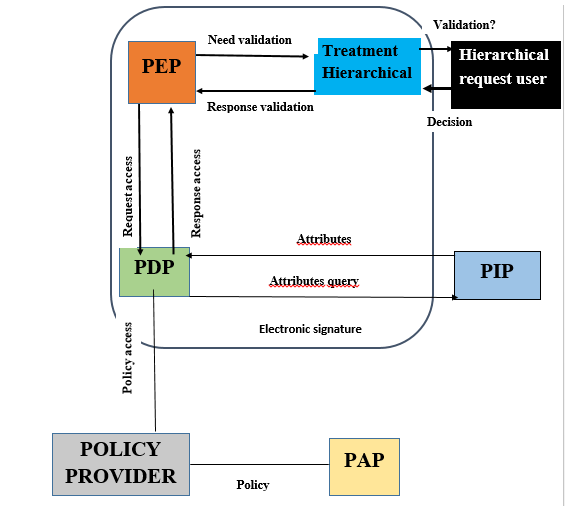
\includegraphics[scale=0.7]{chap4/images/architecture.png}
    \caption{Architecture de notre langage}
	 \label{figArchie}
\end{figure} 

\mySubSection{Modèle de flux de donnée dans notre langage}{}\label{sectionModèle}

notre langage fonctionne comme suite:

\begin{enumerate}
\item Le PAP créer les politiques d'accès et les stocke dans le Policy provider; 
\item Le Policy provider mes les politiques d'autorisation d'accès à la disposition du PDP;
\item L'utilisateur effectue une demande dans le système;
\item Le PEP récupérer la demande d'accès de l'utilisateur la transforme en requête et l'envoie au PDP;
\item Le PDP demande tous les attributs sujet, ressource, action, environnement et autres catégories (non représentés) supplémentaires au PIP;
\item Le PIP obtient les attributs demandés;
\item Le PIP envoie les attributs demandés au PDP;
\item Le PDP évalue la politique;
\item Le PDP renvoie le contexte de réponse (y compris la décision d'accès, la requête et l'obligation qui contient généralement l'unité organisationnelle qui est sensé effectuer un contrôle hiérarchique sur la requête afin de donner la décision d'accès final) au PEP;
\item Le PEP enregistre la requête dans la base de données, évalue l'obligation que contient la réponse
\item Si l'obligation révèle que la requête ne nécessite pas une validation hiérarchique alors, le PEP applique la décision d'accès qui peut être accordée ou refusée;
\item Sinon le PDP envoie la requête au module de traitement hiérarchique; 
\item Le module de traitement hiérarchique évalue la requête et renvoie la décision d'accès au PEP
\item Le PEP notifier l'utilisateur et applique la décision d'accès sur la politique si celle-ci est l'intersection de la décision d'accès renvoyée par le PDP et celle renvoyée par le module de traitement hiérarchique. cette décision peut être "permit" au "refusé".
\end{enumerate}

\begin{figure}[h!]
    \centering
		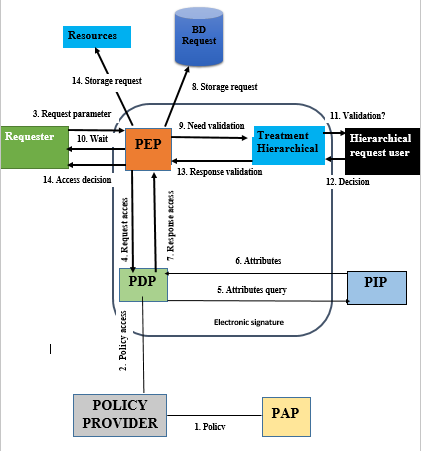
\includegraphics[scale=1.0]{chap4/images/flux.png}
    \caption{Architecture de notre langage}
	 \label{figFluxD}
\end{figure} 

